
\section{Results}

We generate the visibility graph for each sub-region of interest using the time-magnitude sequences shown in Fig.~\ref{fig:mag-time}. The number of nodes in each graph is the same as the (declustered) number of events shown in Table \ref{tab:seismicity}, and the links between inter-visible events are established following the condition in equation (\ref{eq:vg}), as in the example shown in Fig.~\ref{fig:vg}. (We do not include a visualization of the complete sequence graphs because the links are so many, it is only practical to visualize the graphs of short sequences). We then collect information about the number of inter-visibility links associated with each event (connectivity degree, $k$) and categorize the events in magnitude bins of size $\Delta M = 0.1$, as mentioned in the Methodology section. Figure \ref{fig:km} shows the scattered distribution of events in the magnitude-connectivity degree plane for each sub-region. The figure shows that, in general, the value of $k$ increases with $M_w$. Figure \ref{fig:km} also shows the results of obtaining linear $k$-$M$ regressions for each dataset and the values of the $k$-$M$ slopes for the three seismic zones.

\begin{figure*}[t]
	\centering
	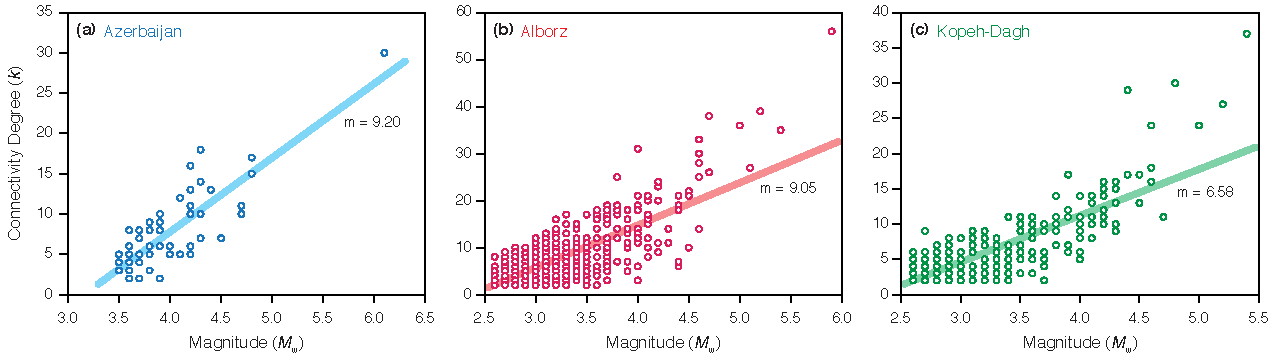
\includegraphics[width=\textwidth]{figures/pdf/figure-06} 
	\caption{Scattered distribution of events in the magnitude-connectivity degree plane and linear regressions obtained for the $k$-$M$ relationships for the three seismic regions in northern Iran. The value next to each of regression line corresponds to the slope of the line, which is referred here as the $k$-$M$ slope. The color version of this figure is available only in the electronic edition.}
	\label{fig:km}
\end{figure*}

Next, we examine the relationship between the $b$-values from Table \ref{tab:seismicity} and the $k$-$M$ slope values shown in Fig.~\ref{fig:km}. Figure \ref{fig:regression} shows the scattered results for $k-M$ slope versus $b$-value for the three tectonic seismic regions in northern Iran along with the data-points obtained for analysis of the magnitude-time sequences of the Mexican subduction zone \citep{Telesca2013} and the Pannoninan seismic zone \citep{Telesca2014}, as well as other experimental results \citep{Telesca2014-pone}. Figure \ref{fig:regression} also include the results of different linear regressions between the $b$-value and the $k$-$M$ slope. Each regression shows the addition of new data-points from different studies over time, with the present study adding the latest set of data. Note that the regression improves as new data-points are added, which is indicated by the correlation coefficient $R$. This was previously pointed out by \citet{Telesca2014}. The values of the correlation coefficients are also shown in the figure. According to these results, the universal relationship between the $b$-value and the $k$-$M$ slope is given by:
% 
\begin{equation}
	b = 000 + 000 m \, 
	\label{eq:universal.bm}
\end{equation}
% 
where $m$ is the value of the $k$-$M$ slope.

\begin{figure}[h]%[t]
	\centering
	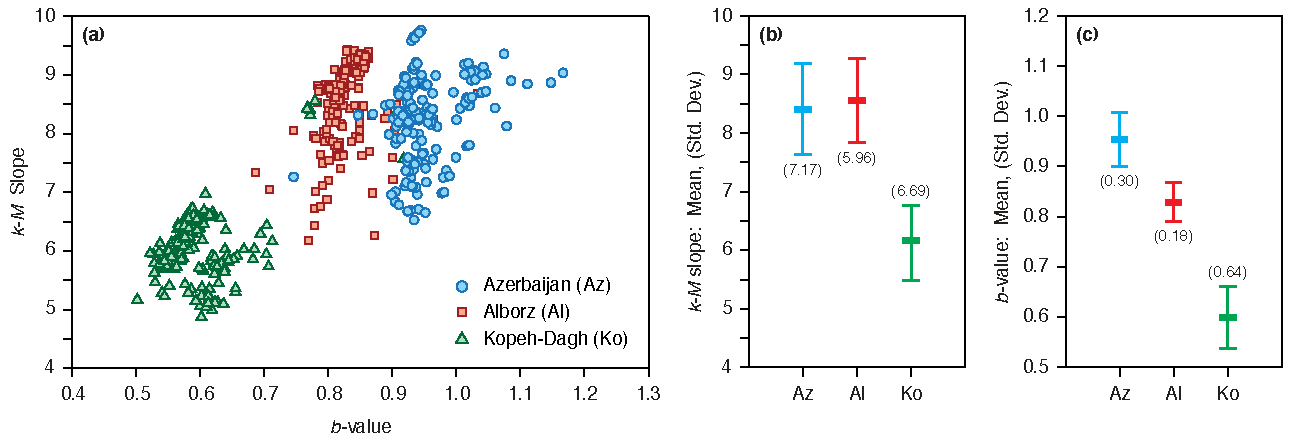
\includegraphics[width=0.45\textwidth]{figures/pdf/figure-07} 
	\caption{Relationship between $k-M$ slope and $b-value$ of three Iranian tectonic seismic zones (this study) and three other studies of Mexican zones \citep{Telesca2013}, Pannonia zones \citep{Telesca2014}, and synthetic data \citep{Telesca2014-pone}. The lines represent the linear regression fit of data. The correlation coefficients (R) are represented for different combination of data.}
	\label{fig:regression}
\end{figure}

The level of correlation indicated by the values of $R$ in Fig.~\ref{fig:regression} being close to 1 is indicative of the stability of the relationship, which could be considered universal provided that future tests continue to reinforce these results. Another aspect of interest is the stability of the data points themselves. Note that as presented in Fig.~\ref{fig:regression}, the analysis of the sequences shown in Fig.~\ref{fig:mag-time} only contribute one data point per sub-region of interest. Furthermore, each data-point comes from sequences that vary significantly in terms of the number of events and seismic parameters. 

\citet{Telesca2013} observed that the value of the $k$-$M$ slope is not particularly sensitive to the sample size in the sequence---at least not when considering sufficiently large sequences. On the other hand, as we will see below, if the sequence window is sufficiently short, then the $k$-$M$ slope value shows a relative dependence on time and thus provides insight about the variation of the seismicity as the sequence progresses. Note also that the threshold value of $M_c$ is significantly smaller for Azerbaijan than for Alborz or Kopeh-Dagh. This is due in part to the fact that the latter two zones were more seismically active in the time period under consideration. However, according to \citet{Telesca2012}, the threshold magnitude has a minor effect in the graph parameters.

To further explore the sensitivity of the graph properties to the number of events in each catalog and the value of the minimum magnitude to be considered, we randomly picked a significant number of sub-sequences from within the initial catalog compiled for each region, and repeated the analysis for each sub-sequence. In total, for each region, we extracted 200 new sub-sequences from the initial (pre-declustering) catalog. The number of events in each sub-sequence was varied randomly but chosen to be large enough to represent the seismic characteristics of each region. In particular, the minimum size of each sub-sequence was set to be $n \geq 150$, whereas the maximum size in the sequence was set to be as large as the original (pre-declustering) catalog. We forced the random sub-sequences to progress positively in time without altering the natural occurrence of events. In other words, we randomly determined the initial event and the sub-sequence size (number of events to be considered), then picked that number of events following the initial earthquake in the sub-sequence. Next, we determined the value of $M_c$ and $b$, created the graph for all events with $M \geq M_c$, and extracted the connectivity degree of the events in each sub-sequence. 

Figure \ref{fig:random}a shows scattered points for all the individual $k$-$M$ slope and $b$-value pairs for all the sub-sequences that were randomly generated for each region in northern Iran. Next to it, Figs.~\ref{fig:random}b and \ref{fig:random}c show the 

The figure also shows the linear correlation for the 

the relationship between  $k-M$  slope and  $b-value$  of the randomly selected data and the statistical parameters for variables. Although changing the number of events and the threshold magnitude is slightly changing the results, however,  the results are fairly well clustered for each tectonic seismic region. 

% =========

% We compared the $k$-$M$ slope with the $b$-value of the Gutenberg-Richter law through the entire catalog and in the sliding windows in time. 

% Comparing the result with the Guerrero region with reduced random sequence,  \citet{Telesca2013}  found that the number of sequences did not affect the $k-M$ slope.

% Fig.~\ref{fig:random} shows the relationship between  $k-M$  slope and  $b-value$  of the randomly selected data and the statistical parameters for variables. Although changing the number of events and the threshold magnitude is slightly changing the results, however,  the results are fairly well clustered for each tectonic seismic region. 
   
% The coefficient of variation of parameters is shown in Fig.~\ref{fig:random}. The  $k-M$  slope shows the higher coefficient of variation which indicates the fact that the  $k-M$  slope is more dependent on the window size and threshold magnitude than on the a-  and  b-values , which suggests that  the $k-M$  slope can better represent the dynamic characteristics of the magnitude-time series. 

\begin{figure*}%[t]
	\centering
	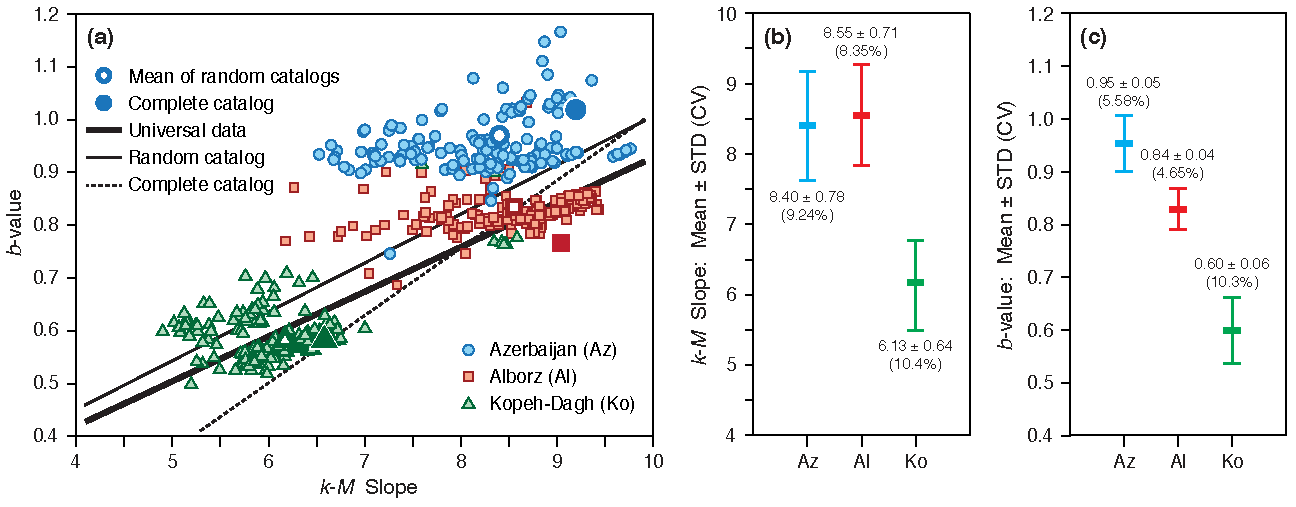
\includegraphics[width=0.9\textwidth]{figures/pdf/figure-08} 
	\caption{Relationship between $k-M$ and $b-value$ of three Iranian tectonic seismic regions for 200 random sequence. The numbers on the mean and standard deviation plots are coefficient of variations in percent $(standard \ deviation / mean)$.}
	\label{fig:random}
\end{figure*}

% *******

% Fig.\ref{fig:tc} shows the variation of the  $k-M$  slope and  $b-value$  with time. Due to lower number of events in Azerbaijan's catalog, we choose 20 events as the window length with a shift of one event between two successive windows. With higher window length we loose the variation of considerable amount of information in time (e.g. with n=40 we loose almost half of the Azerbaijan catalog). Due to taking average values of successive windows, very small window length can not display the seismicity behavior especially before big earthquake. Maintaining consistency, we use the window length equal to 20 events for all three regions. The calculated parameters of each window are associated with the time of occurrence of the last event in the sliding window. The  $k-M$  slope and  $b-value$  in all tectonic seismic regions are very similar. In general, in all regions the $b-value$  and  $k-M$  slope drop considerably before large earthquakes. The decline in the  $b-value$  before large earthquakes has been studied in many regions \citep{Wyss2000, Wyss2006, Schorlemmer2005, Chan2012}.

% \citet{Telesca2016}  observed the decrease in  $<T_c>$  before the large earthquake of the western India earthquake sequence. Fig.\ref{fig:tc}  shows the time variation of  $<T_c>$   in the study area. The reduction of  $<T_c>$   before large earthquakes is clearly visible.  \citet{Telesca2016}  demonstrated that the decrement of  $<T_c>$   before a large earthquake is independent of window size and threshold magnitude. Decreasing the value of  $<T_c>$  ,  $k-M$ , and  $b-value$  before large earthquakes predominantly happened in all tectonic seismic regions (see Fig.\ref{fig:tc} for reference.)
 
\begin{figure*}[t]
	\centering
	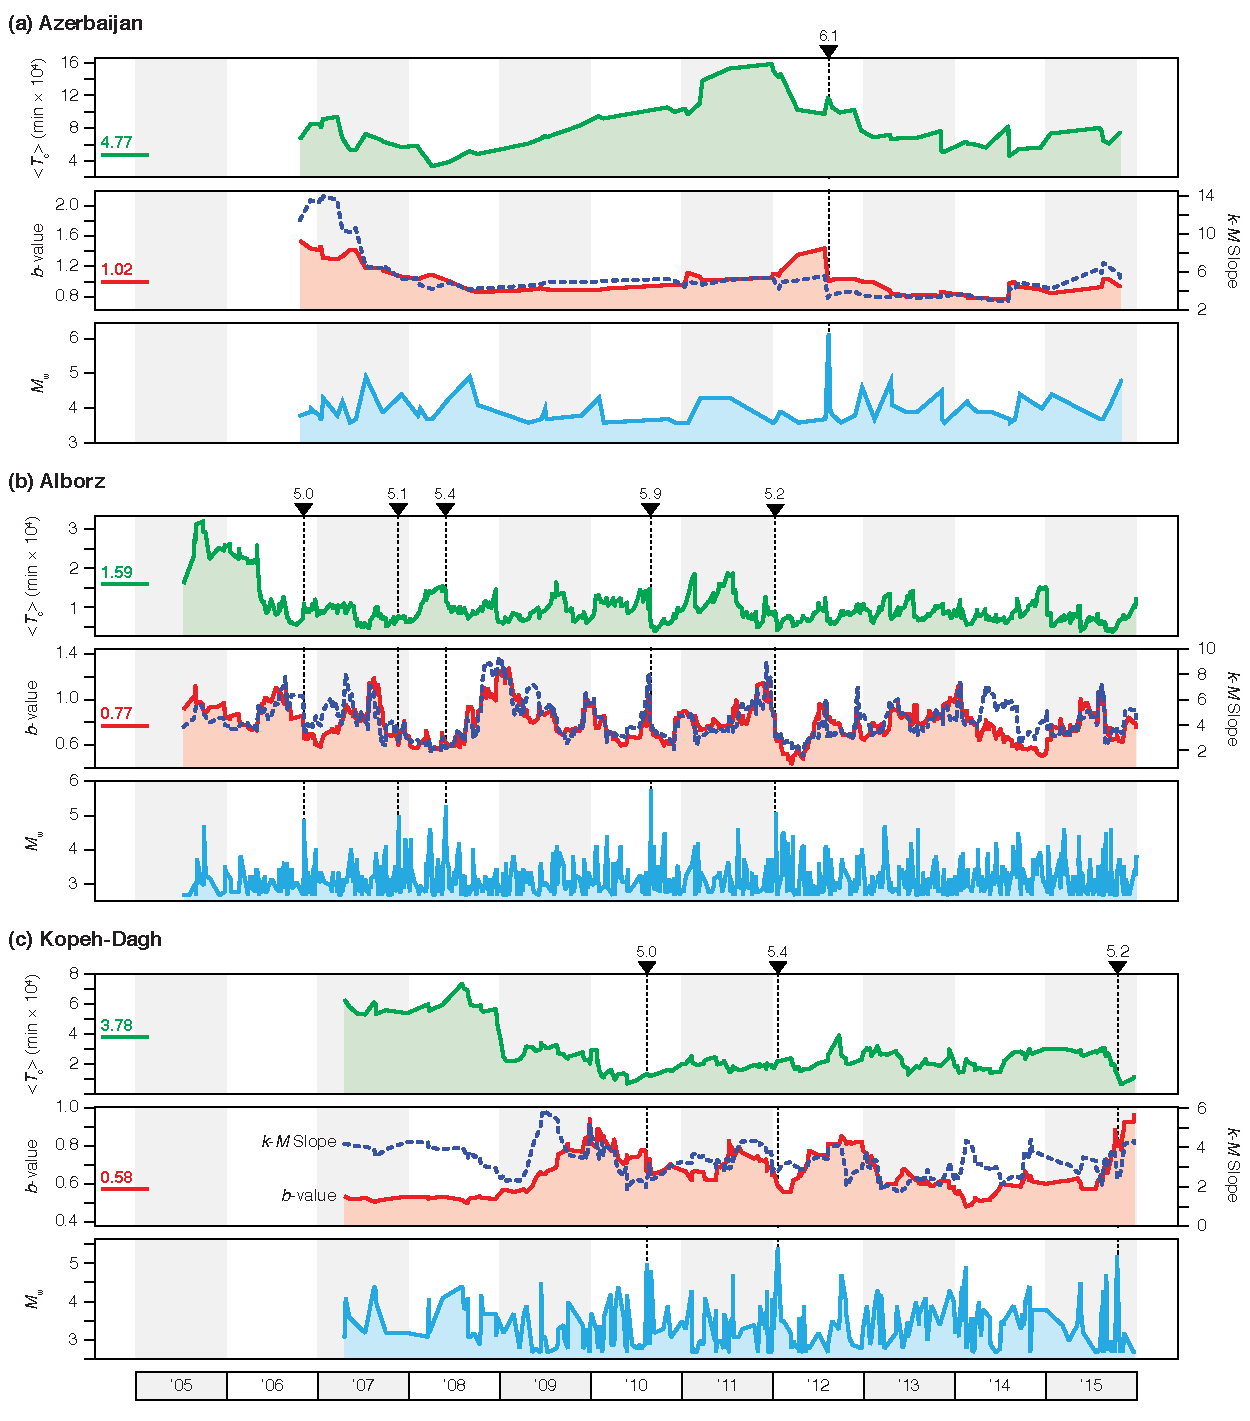
\includegraphics[width=\textwidth]{figures/pdf/figure-09} 
	\caption{ Variation of $k-M$ slope  and $b-value$ (Left), and $ < T_c >$ (Right) as a function of time for three tectonic seismic regions in north Iran. Black arrows show the occurrence of the major earthquakes. Numbers on arrows indicate the moment magnitude of the earthquake (see Fig.~\ref{fig:mag-time} for reference).  The magnitude-time series are presented as a filled plot blew each plot. The variation of the heigh of filled plots are corresponding to the event magnitudes. Decreasing the value of  $<T_c>$  ,  $k-M$ , and  $b-value$  before large earthquakes predominantly happened in all tectonic seismic regions.}
	\label{fig:tc}
\end{figure*}
